% uploaded from https://www.latextemplates.com/template/pnas
%%%%%%%%%%%%%%%%%%%%%%%%%%%%%%%%%%%%%%%%%
% Proceedings of the National Academy of Sciences (PNAS)
% LaTeX Template
% Version 1.0 (19/5/13)
%
% This template has been downloaded from:
% http://www.LaTeXTemplates.com
%
% Original author:
% The PNAStwo class was created and is owned by PNAS:
% http://www.pnas.org/site/authors/LaTex.xhtml
% This template has been modified from the blank PNAS template to include
% examples of how to insert content and drastically change commenting. The
% structural integrity is maintained as in the original blank template.
%
% Original header:
%% PNAStmpl.tex
%% Template file to use for PNAS articles prepared in LaTeX
%% Version: Apr 14, 2008
%
%%%%%%%%%%%%%%%%%%%%%%%%%%%%%%%%%%%%%%%%%

%----------------------------------------------------------------------------------------
%	PACKAGES AND OTHER DOCUMENT CONFIGURATIONS
%----------------------------------------------------------------------------------------

%------------------------------------------------
% BASIC CLASS FILE
%------------------------------------------------

%% PNAStwo for two column articles is called by default.
%% Uncomment PNASone for single column articles. One column class
%% and style files are available upon request from pnas@nas.edu.

%\documentclass{pnasone}
\documentclass{pnastwo}

%------------------------------------------------
% POSITION OF TEXT
%------------------------------------------------

%% Changing position of text on physical page:
%% Since not all printers position
%% the printed page in the same place on the physical page,
%% you can change the position yourself here, if you need to:

% \advance\voffset -.5in % Minus dimension will raise the printed page on the 
                         %  physical page; positive dimension will lower it.

%% You may set the dimension to the size that you need.

%------------------------------------------------
% GRAPHICS STYLE FILE
%------------------------------------------------

%% Requires graphics style file (graphicx.sty), used for inserting
%% .eps/image files into LaTeX articles.
%% Note that inclusion of .eps files is for your reference only;
%% when submitting to PNAS please submit figures separately.

%% Type into the square brackets the name of the driver program 
%% that you are using. If you don't know, try dvips, which is the
%% most common PC driver, or textures for the Mac. These are the options:

% [dvips], [xdvi], [dvipdf], [dvipdfm], [dvipdfmx], [pdftex], [dvipsone],
% [dviwindo], [emtex], [dviwin], [pctexps], [pctexwin], [pctexhp], [pctex32],
% [truetex], [tcidvi], [vtex], [oztex], [textures], [xetex]

\usepackage{graphicx}

%------------------------------------------------
% OPTIONAL POSTSCRIPT FONT FILES
%------------------------------------------------

%% PostScript font files: You may need to edit the PNASoneF.sty
%% or PNAStwoF.sty file to make the font names match those on your system. 
%% Alternatively, you can leave the font style file commands commented out
%% and typeset your article using the default Computer Modern 
%% fonts (recommended). If accepted, your article will be typeset
%% at PNAS using PostScript fonts.

% Choose PNASoneF for one column; PNAStwoF for two column:
%\usepackage{PNASoneF}
%\usepackage{PNAStwoF}

%------------------------------------------------
% ADDITIONAL OPTIONAL STYLE FILES
%------------------------------------------------

%% The AMS math files are commonly used to gain access to useful features
%% like extended math fonts and math commands.

\usepackage{amssymb,amsfonts,amsmath}

%------------------------------------------------
% OPTIONAL MACRO FILES
%------------------------------------------------

%% Insert self-defined macros here.
%% \newcommand definitions are recommended; \def definitions are supported

%\newcommand{\mfrac}[2]{\frac{\displaystyle #1}{\displaystyle #2}}
%\def\s{\sigma}

%------------------------------------------------
% DO NOT EDIT THIS SECTION
%------------------------------------------------

%% For PNAS Only:
\contributor{Submitted to Proceedings of the National Academy of Sciences of the United States of America}
\url{www.pnas.org/cgi/doi/10.1073/pnas.0709640104}
\copyrightyear{2008}
\issuedate{Issue Date}
\volume{Volume}
\issuenumber{Issue Number}

%----------------------------------------------------------------------------------------

\begin{document}

%----------------------------------------------------------------------------------------
%	TITLE AND AUTHORS
%----------------------------------------------------------------------------------------

%\title{Title of the publication} % For titles, only capitalize the first letter
\title{Health implications of smoke from prescribed fires and wildfires} % For titles, only capitalize the first letter
%------------------------------------------------

%% Enter authors via the \author command.  
%% Use \affil to define affiliations.
%% (Leave no spaces between author name and \affil command)

%% Note that the \thanks{} command has been disabled in favor of
%% a generic, reserved space for PNAS publication footnotes.

%% \author{<author name>
%% \affil{<number>}{<Institution>}} One number for each institution.
%% The same number should be used for authors that
%% are affiliated with the same institution, after the first time
%% only the number is needed, ie, \affil{number}{text}, \affil{number}{}
%% Then, before last author ...
%% \and
%% \author{<author name>
%% \affil{<number>}{}}

%% For example, assuming Garcia and Sonnery are both affiliated with
%% Universidad de Murcia:
%% \author{Roberta Graff\affil{1}{University of Cambridge, Cambridge,
%% United Kingdom},
%% Javier de Ruiz Garcia\affil{2}{Universidad de Murcia, Bioquimica y Biologia
%% Molecular, Murcia, Spain}, \and Franklin Sonnery\affil{2}{}}

\author{John Smith\affil{1}{University of California},
James Smith\affil{2}{University of Oregon}
\and
Jane Smith\affil{1}{}}

\contributor{Submitted to Proceedings of the National Academy of Sciences
of the United States of America}

%----------------------------------------------------------------------------------------

\maketitle % The \maketitle command is necessary to build the title page

\begin{article}

%----------------------------------------------------------------------------------------
%	ABSTRACT, KEYWORDS AND ABBREVIATIONS
%----------------------------------------------------------------------------------------

\begin{abstract}
[Starting text from NASA proposal, need to differentiate from PM2.5 surface paper]

Wildfires in the western US are increasing both in terms of acres burned and economic impact. Prescribed fires are used as a management tool to reduce fuel loads and the risk of large uncontrolled wildfires while allowing ecological benefits of fire. Previous research indicates that prescribed fires impact air quality less than wildfires on a per-fire basis. To our knowledge, previous studies have not considered if air pollution from prescribed fires and wildfires pose differential risks to public health. Air quality managers and public health professionals in the western US want empirical evidence of the health impacts associated with prescribed fires to inform their smoke management plans and public health interventions and messaging. Prescribed fires often occur in more rural areas, thus large datasets over broad geographic areas for many years are needed for statistical power, and studies cannot rely solely on monitoring data for air pollution exposure estimation as these monitors are often far from fire-impacted areas. Increasingly, researchers are statistically blending information from remotely-sensed Earth observations, atmospheric models, and air quality monitoring data to obtain improved spatiotemporal air pollution exposure surfaces for health studies. Our proposal directly fits within the NASA Health and Air Quality Area objectives of incorporating Earth observations into air quality management and public health. Our project has three aims. 

We will use surface PM2.5 estimates obtained from machine learning algorithms to analyze the associations of fire-attributed PM\textsubscript{2.5} levels with cardiorespiratory health endpoints to determine if the health impacts associated with prescribed fire smoke are different from those of wildfire smoke. To our knowledge, our work will be the first to (1) assess health impacts associated with prescribed fire smoke and (2) analyze cardiorespiratory impacts of repeated smoke exposures.
\end{abstract}

%------------------------------------------------

\keywords{Keyword1 | Keyword2 | Keyword3} % When adding keywords, separate each term with a straight line: |

%------------------------------------------------

%% Optional for entering abbreviations, separate the abbreviation from
%% its definition with a comma, separate each pair with a semicolon:
%% for example:
%% \abbreviations{SAM, self-assembled monolayer; OTS,
%% octadecyltrichlorosilane}

% \abbreviations{}
\abbreviations{air pollution}

%----------------------------------------------------------------------------------------
%	PUBLICATION CONTENT
%----------------------------------------------------------------------------------------

%% The first letter of the article should be drop cap: \dropcap{} e.g.,
%\dropcap{I}n this article we study the evolution of ''almost-sharp'' fronts

\section{Introduction}

%\dropcap{N}am fermentum sapien at enim varius consectetur. Quisque lobortis imperdiet mauris, et accumsan libero vulputate vitae. Integer lacinia purus vel metus tempus suscipit. Curabitur ac sapien quis mauris euismod commodo. Sed pharetra sem elit. Fusce ultrices, mauris eu fermentum tempor, tellus sem ornare lectus, in convallis nunc urna id dolor. Donec convallis ligula vitae sem viverra fermentum. Mauris in ullamcorper erat. Donec ultrices tempus nibh quis vestibulum. This statement requires citation \cite{CLAcha1}.

[Use dropcap code on first letter of paragraph]

Knowledge about the health impacts associated with fine particulate matter (PM\textsubscript{2.5}) from fires is important for air quality managers and  public health departments, particularly in western US states where fire can often cause public health and air quality emergencies. We have therefore partnered with the Western States Air Resources (WESTAR) Council, and the Centers for Disease Control and Preparedness’s Environmental Public Health Tracking Network (EPHTN), as the results of our proposed work would be useful to their state partners.

Air quality is managed at the state and local levels to conform to air quality standards set by state and federal policy. Decisions about when to set prescribed fires involve air quality management agencies for states, tribal, and sometimes local areas in order to mitigate impacts that are both regulated and of concern for public health. State and local land management agencies are tasked with writing smoke management plans whenever they put fire on the ground \cite{SmokeManagement2001}. Smoke plans involve planning burns that produce minimal smoke with maximum ecological benefit and fit within specific land management plans that consider the benefits of fire while minimizing risks related to both fire and smoke. Prescribed fire planning involves modeling both the quantity and trajectories of emissions from the proposed prescribed fire with smoke prediction tools. When projected emission levels are lower than the air quality standard for fine particulate matter (PM\textsubscript{2.5}), it is assumed that there are no health impacts, however, it is possible that health impacts could occur at that level or lower. Furthermore, sometimes air pollution levels from prescribed fires reach levels higher than smoke planning tools predict. 

Fire is a necessary part of many ecosystems in the western US, and complete fire suppression is not feasible. To help minimize risk of often catastrophic unplanned wildfires, prescribed burning is used to reduce fuels and create desired ecosystem conditions. There are tensions among various stakeholders involved in land, fire, air quality, and public health management with some wanting to do more prescribed burning and some wanting to do less. In different states, the public can be on either side of this issue. State air quality managers have impressed upon us that they are incredibly supportive of this project because it will provide them with data on the health impacts of prescribed fires and wildfires that they can present to various stakeholders to base these discussions on science more than on the presumed benefits of more or less prescribed fire. Our project is timely as the state of Oregon is undergoing review of their smoke management plan, and other states will be reviewing their smoke management plans in the near future. The results of our proposed project can inform these processes. Better understanding of health impacts associated with exposure to smoke from wildfires and prescribed fires could allow better planning for future prescribed burning and targeted mitigation strategies in the face of unplanned wildfire events.

Our partners at WESTAR have indicated to us that their organization, and particularly the state air quality managers who form their organization, are interested in understanding the concentration-response functions for PM\textsubscript{2.5} from various types of fire. They are especially interested in understanding if there is a difference in the health impacts of PM\textsubscript{2.5} from prescribed fires versus unplanned wildfires. They will use this information as part of their smoke management planning, which many of our state partners are updating in the next few years.

EPHTN’s mandate is to collect, integrate, and analyze non-infectious disease and environmental data for empowering environmental and public health practitioners, health-care providers, community members, policy-makers, and others to make information-driven decisions that affect health \cite{AboutCDCtracking2017}. We have partnered with EPHTN because their partners, state public health departments, are interested in knowing more about air pollution exposures attributable to various types of fires and understanding the health risks associated with those exposures. 

The current advice for public health departments on how to protect the public from wildfire smoke does not refer to prescribed fires \cite{EPA2016}. The reason for no differentiated communication to the public is because there is currently no information on the association between smoke from prescribed fires and health, so it is assumed to be the same as that from wildfires, and only impacted by the level of PM\textsubscript{2.5}. Public health officials are encouraged to use the Air Quality Index (AQI) (a tool to communicate air pollution levels to the public) to recommend health protective actions such as using an air filter and staying indoors. If differential health impacts of PM\textsubscript{2.5} associated with prescribed fire or wildfire smoke at levels below 
%35 \textmu g/m\textsuperscript{3}
(the current 24-hour PM\textsubscript{2.5} standard set by the US EPA) are found to occur, then more targeted messages could be made that may help protect the public 
from an exposure that is a part of our ecosystem and cannot be removed. 

% * <melissa.maestas@colorado.edu> 2017-11-29T22:13:29.964Z:
% 
% fix that it crashes when line 219 is uncommented
% 
% ^.

Our state public health partners have indicated to us that they will use the results of our study to provide information to the public to increase the understanding of wildfire (or prescribed fire) and how it can impact health, in general. They will use the information to more effectively target their public health messages should a differential health effect between wildfire smoke and prescribed fire smoke be found. In communities in which there is a lot of opposition to prescribed burns, they would like to quantify the impact of wildfires versus prescribed fires using the results from our study. This may increase their ability to get the public’s support in targeted communities while also motivating them to take steps to reduce exposure when a prescribed burn is scheduled. The state public health departments measure baseline performance as the daily PM\textsubscript{2.5} from monitoring stations as well as the number of respiratory and cardiovascular hospitalizations, emergency department visits, and deaths on days with wildfire smoke. Ultimately, their goal is to reduce emergency department and hospitalization visits for respiratory and cardiovascular conditions on these days. 

In addition to information about the associations between cardiovascular and respiratory health and PM\textsubscript{2.5} from wildfires and prescribed fires, we will provide fire-type source-apportioned annual estimates of PM\textsubscript{2.5} concentrations at the county level for the western US to EPHTN. The state partners of EPHTN can use these annual estimates for further investigations of the health impacts of smoke from wildland fires in their own communities, using more local information on health that cannot be provided to outside researchers. This will continually enhance the decision-making of public health departments in the western US related to communicating about health interventions for high smoke events from wildfires and prescribed fires.

Both the annual estimates and the daily ZIP code-level PM\textsubscript{2.5} estimates will be made publicly available via the EPHTN national portal \url{https://ephtracking.cdc.gov/DataExplorer/} as well as state EPHTN portals to enable members of the public, including environmental and public health practitioners, healthcare providers, community members, policy-makers, and others to make connections between the environments where they live and their health. 

The increase in frequency and severity of landscape fires occurring in the western US \cite{Dennison2014,Steel2014} and the decrease in other sources of air pollution 
%\cite{EPAPM25Trends2017} mean that smoke from landscape fires will be an increasingly large 
fraction of total air pollution. The increase in wildfires has prompted increasing pressure to engage in more prescribed burning \cite{Stephens2005}. Therefore, understanding (1) the exposure of the public to air pollution from wildfires and prescribed fires and (2) the impacts of smoke exposure from both prescribed fires and wildfires on health are important and timely topics, which are addressed in this project.

% * <melissa.maestas@colorado.edu> 2017-11-29T22:27:23.945Z:
% 
% Fix it so it doesn't crash when line 236 is uncommented.
% 
% ^.

Increasingly, in the wildfire-health literature, researchers are `blending' satellite AOD data and air quality models together to estimate air quality exposures in locations far from monitoring sites, (e.g., \cite{Reid2016EnvRes,Reid2015,vanDonkelaar2011,Gan2017}) as these two data sources have different strengths and weaknesses but merged together can better estimate exposures. Satellite AOD data is a measurement but of the full atmospheric column rather than at ground level, whereas ground-level PM\textsubscript{2.5} estimates can be extracted from air quality models, but there are uncertainties inherent in the models. Blending these data sources over large geographic areas and long periods of time, including many fires in different locations, can provide the statistical power needed to detect if there are differential health impacts from smoke from prescribed fires and unplanned wildfires.

Air quality managers and public health departments work together to protect public health from air pollution due to prescribed burns, but that proves difficult without knowing if the health impacts for this fire type are different from those for wildfires. Therefore, we are partnering with the Western States Air Resources Council (WESTAR) and the Environmental Public Health Tracking Network (EPHTN) of the Centers for Disease Control and Prevention to operationalize our research to support decision-making by states about how to minimize health impacts from prescribed fires and wildfires. 

Our proposal aims to address this gap in knowledge by addressing the following objectives:

\begin{enumerate}
\item Estimate the proportion of total 
PM\textsubscript{2.5} per day attributed to all sources, and then specifically for wildfires and prescribed fires. This will entail the following steps:
\begin{enumerate}
\item Create a multi-year daily spatiotemporal total PM\textsubscript{2.5} exposure surface for an 11-state area in the western US for the years 2008-2014
\item Model the transport of air pollutant emissions from each fire type (wildfire and prescribed fire), daily for the study area
\item Calculate daily estimates of wildfire-attributed and prescribed fire-attributed PM\textsubscript{2.5} for all ZIP codes in the study area for all 7 years
\end{enumerate}
\item Calculate annual average PM\textsubscript{2.5} concentrations for each fire type and total for each county in the 11-state area for use by EPHTN
\item Analyze the associations of PM\textsubscript{2.5} from each fire type on respiratory and cardiovascular hospitalizations and mortality 
\item Disseminate results about the differential health impacts of wildfire PM\textsubscript{2.5} and prescribed fire PM\textsubscript{2.5} on respiratory and cardiovascular health to WESTAR and EPHTN for use in their decision-making related to air quality and health impacts of prescribed fires and wildfires
\end{enumerate}

Fire is an integral part of many ecosystems, yet many fires are suppressed to protect human populations, property, and infrastructure \cite{Bowman2009}. This suppression can lead to a build-up of fuels that contribute to the increased intensity of wildfires in the western US \cite{Schoennagel2017}. Prescribed fires are used as a management tool to decrease fuel loads and risk of large uncontrolled wildfires while allowing for the ecological benefits of fire \cite{Schoennagel2017}. Previous research indicates that prescribed fires may impact air quality less than wildfires on a per-fire basis \cite{Liu2017}. In planning prescribed fire, air quality managers are obligated to understand and plan for the impacts of smoke on air quality and to minimize the impact of smoke on populations (see more from the National Interagency Fire Center at \url{https://www.nifc.gov/smoke/index.html}). Prescribed fires, therefore, are intended to last for short durations and under ideal weather conditions for allowing smoke to be transported away from settlements, making it less of a concern than wildfires which often burn under adverse conditions for smoke management. Currently, there is tension between entities that want more prescribed fires and those who oppose them, who often cite air quality and health concerns as their primary opposition to prescribed fires. Air quality managers are often caught in the middle. Empirical information on the health impacts of historical prescribed fires, which is not currently available, could help quantify the benefits of prescribed burning and scientifically inform the ongoing debate about whether it is prudent to increase prescribed burning in the western US.

A differential risk for health for prescribed fires is plausible because prescribed fires 
(1) typically burn at lower temperatures with more smoldering than high intensity wildfires which can lead to differences in chemical composition of emissions, 
%\citep{Torvela2014}, 
(2) tend to occur during different times of the year than wildfires, and this could lead to burning wetter fuels, affecting particle chemistry and quantity, %\citep{WilliamsonTransdisciplinary2016}, 
(3) are lower intensity which can lead to lower atmospheric injection height and therefore more air quality impacts where people breathe, and %\citep{WilliamsonTransdisciplinary2016}, and 
(4) have to be repeatedly set to have an impact on controlling larger fires, 
potentially leading to more chronic exposure to smoke % added this line
\cite{WilliamsonTransdisciplinary2016,Torvela2014}. %\citep{WilliamsonTransdisciplinary2016}. 
Thus, although studies have documented lower air pollution levels from prescribed fires \cite{Liu2017}, it is not clear that the health impacts would be less than those caused by wildfires. 

To understand if there are differential health impacts of smoke from prescribed fires and wildfires on population health, a very large dataset needs to be created and analyzed. We therefore propose to create estimates of PM\textsubscript{2.5} source-apportioned to each fire type for a 7-year period (2008-2014) over an 11-state region of the western US (see Figure \ref{fig:Map11States}). To date, there have been no empirical studies of the health effects of prescribed fires compared to wildfires, despite some theoretical publications \cite{Haikerwal2015JAWMA,SchweizerForest2017} 
on the important considerations related to these two sources of air pollution that are increasing in importance in the western US. Therefore, our study will be ground-breaking in its ability to attribute fine particulate matter, both emitted (primary PM\textsubscript{2.5}) and chemically-created (secondary PM\textsubscript{2.5}), to wildfires and prescribed fires in the historical record and then to estimate the health impacts from these fire types on cardiovascular and respiratory health outcomes among the elderly, a particularly sensitive subpopulation about which we have a consistent national dataset. 

The results from these studies will be important not just for furthering the science of the health implications of wildfire and prescribed fire smoke, but will also be used by decision makers in both air quality management and public health, as evidenced by our letters of support from WESTAR and EPHTN. The state partners of these groups have expressed enthusiastic support for our project with intent to use our results for current and future smoke and public health preparedness planning. 

We will also pilot the first, to our knowledge,
investigation into the health impacts of repeated exposures to smoke from prescribed fires and wildfires. 


%\begin{equation}
%\mfrac{D \theta}{Dt}=\mfrac{\pr \theta}{\pr t} + u\cdot \nabla
%\theta=0 \label{qg1}
%\end{equation}

%Referencing equation \eqref{qg1}. Praesent volutpat, nibh in dignissim commodo, tellus justo consequat erat, vel consequat mi arcu vel lectus. Aliquam a tellus nec felis sagittis consequat. Quisque convallis imperdiet neque a tempor. Nulla non erat urna. Mauris vel lorem magna, tristique auctor ipsum. Aliquam pharetra eleifend massa. Donec porttitor sagittis luctus. Aliquam pretium luctus leo quis congue. Morbi vel felis mi. Suspendisse viverra tortor pretium orci lacinia eleifend. Phasellus aliquam, nunc eu cursus feugiat, erat odio porttitor libero, quis accumsan orci ipsum ut lorem. Vestibulum pharetra malesuada egestas. Sed non orci sit amet erat suscipit fringilla in et diam. Vestibulum ante ipsum primis in faucibus orci luctus et ultrices posuere cubilia Curae; Nunc ut rhoncus nulla. Aenean porta rhoncus suscipit.

%------------------------------------------------

\section{Results}

Mauris vel lorem magna, tristique auctor ipsum. Aliquam pharetra eleifend massa. Donec porttitor sagittis luctus. Aliquam pretium luctus leo quis congue. Morbi vel felis mi. Referencing Table \ref{sampletable}. Referencing Figure \ref{placeholder}.

\subsection{Simulations}

\subsubsection{Simulation 1}

Vivamus magna enim, aliquet id cursus a, pharetra ut purus. Phasellus suscipit nisi iaculis mi vulputate id interdum velit dictum. Nam ullamcorper elit in lectus ultrices vitae volutpat massa gravida. Etiam sagittis commodo neque eget placerat. Sed et nisi faucibus metus interdum adipiscing id nec lacus. Donec ipsum diam, malesuada at euismod consectetur, placerat quis diam. Phasellus cursus semper viverra. Proin magna tortor, blandit in ultricies id, facilisis at nibh. Proin eu neque est. Etiam euismod auctor ante. Mauris mauris sem, tincidunt a placerat rutrum, porta id est. Aenean non velit porta eros condimentum facilisis at in nibh. Etiam cursus purus ut orci rhoncus sit amet semper eros porttitor. Etiam ac leo at ipsum tincidunt consequat ac non sapien. Aenean sed leo diam, venenatis pharetra odio.

\subsubsection{Simulation 2}

Suspendisse viverra eleifend nulla at facilisis. Nullam eget tellus orci. Cras sit amet lorem velit. Maecenas rhoncus pellentesque orci eget vulputate. Phasellus massa nisi, mattis nec elementum accumsan, blandit non neque. In ac enim elit, sit amet luctus ante. Cras feugiat commodo lectus, vitae convallis dui sagittis id. In in tellus lacus, sed lobortis eros. Phasellus sit amet eleifend velit. Duis ornare dapibus porttitor. Maecenas eros velit, dignissim at egestas in, tincidunt lacinia erat. Proin elementum mi vel lectus suscipit fringilla. Mauris justo est, ullamcorper in rutrum interdum, accumsan eget mi. Maecenas ut massa aliquet purus eleifend vehicula in a nisi. Fusce molestie cursus lacinia.

\subsection{Real Data}



%------------------------------------------------

\section{Discussion}

general reference for health effects of PM2.5 and O3 (non-wildfire) \cite{Cromar2018}... see references \#42-47 therein about health effects of wildfire smoke and compare those to our study

[text from NASA grant as starting point:]

This work directly addresses NASA's desire to ``discover and demonstrate innovative and practical uses of Earth observations'' by using several Earth observations, including several MODIS, Landsat, and VIIRS products, to spatiotemporally estimate ground-level PM\textsubscript{2.5} concentrations and combine this information with Medicare data so that we may better understand the health impacts of smoke from both prescribed fires and wildfires in the western US. Using satellite data and other Earth observations allows us to estimate air quality in locations without air quality monitors. \textbf{Our results will be used by both state air quality managers in updating their smoke management plans and state health departments for targeted communication related to health-protective measures during prescribed fires and wildfires.} All of this work is directly applicable to NASA's Health and Air Quality Application area's interest in the use of Earth observations in air quality management and public health. By working with the NASA Earth Science Division (ESD)/Applied Sciences socioeconomic consortium to coordinate our research and results, the work proposed could be of interest to other NASA Applied Sciences activities.

Our work falls under NASA's Second Strategic Goal in the 2014 Strategic Plan to ``advance understanding of Earth and develop technologies to improve the quality of life on our home planet'' within the realm of Objective 2.2 to ``advance knowledge of Earth as a system to meet the challenges of environmental change, and to improve life on our planet.'' Wildfires are a significant source of air pollution that impacts the health of human populations, particularly in the western US. Prescribed fires are one way to decrease high-intensity catastrophic fires, but without empirical knowledge of the health impacts of prescribed fires compared to wildfires, it is difficult for all stakeholders to come to consensus about the use of prescribed fires. 
Our work will inform how the western US decides to manage its forests to minimize health harms from ecologically necessary fires on the landscape. 

The relevance of our work to decision-makers in both air quality and public health is apparent by the \textbf{incredible outpouring of support we have received from WESTAR and EPHTN as well as their state partners}. This is exemplified in the letters of support that are part of our proposal submission. We had more letters of support than we were allowed to submit with this application, thus EPHTN and WESTAR leaders offered to compile one letter of support from all of their state partners who were interested. The WESTAR letter of support implies that all state air quality managers provide their support, even though they are not enumerated. We also received individual letters of support from some air quality managers before they knew about the combined WESTAR letter. We have included the letter from Colorado as an example of these letters that we also received from New Mexico and Washington. 

\section{Anticipated Results and Improvements}
% 1 page
% This section describes the expected results and improvements to the decision-making activity from the application and integration of Earth observations. This section should articulate the expected improvement(s) over the "baseline" performance of the decision-making activity.

%[paragraph re-write below]Many state smoke management programs were put into place to assist states with implementing measures to reduce regional haze. Smoke management and difficulties communicating across agencies is often seen as an impediment to more prescribed fires in the US \citep{SneeuwjagtOpportunities2013}. In addition to this, decisions about when and where to set prescribed burns is done based on air quality, but without information related to the health impacts associated with smoke from wildfires and prescribed fires; these decisions are being done without complete information. Thus the baseline performance of these decisions is based on a presumption that if the air quality impacts of the prescribed fire are low, then the health impacts will also be low. According to our state partner collaborators, no information on health associated with changes in air quality is known but just assumed because no one has yet done an analysis such as the one presented here. 
Many state smoke management programs were put into place to assist states with implementing measures to reduce regional haze. Smoke management and difficulties communicating across agencies are often seen as impediments to more prescribed fires in the US \cite{SneeuwjagtOpportunities2013}. In addition to this, decisions about when and where to set prescribed burns are made based on air quality, but without information related to the health impacts associated with smoke from wildfires and prescribed fires. Since these decisions are being made without complete information, the baseline performance of these decisions is based on a presumption that if the air quality impacts of the prescribed fire are low, then the health impacts will also be low. According to our state partner collaborators, no information on health impacts associated with smoke from prescribed fires is known but just assumed because no one has yet done an analysis such as the one presented here. 

The state partners are enthusiastic about this project because it will provide them with information to influence their smoke management planning and public health messaging. For example, if we find that there are significant health impacts of prescribed fires at levels below the national ambient air quality standard, this could cause smoke management plans to modify the use of prescribed fires to have lower impacts on air quality. On the other hand, if we find that there are no significant health impacts from prescribed fires, or that they begin to occur at higher levels of PM\textsubscript{2.5}, then smoke management plans may be modified to allow more burning. Similarly in regards to public health decision-making, more targeted messaging for how to protect oneself during fires could be employed for different types of fires if there are indeed differential health impacts. Currently, messaging is the same regardless of fire type \cite{EPA2016}. %change this last refernce to see this for more information on recommendations for public health messaging for wildfires smoke. 
% not sure what to put here. A few ideas:
% \citep{Olsen2017} - about public acceptance of various fire types - https://doi.org/10.1071/WF16034
% https://www.epa.gov/air-research/wildfire-smoke-and-health-risk-communication-workshop-and-report ... featured talk by Olsen
% https://www.epa.gov/air-research/wildland-fire-research-health-effects-research

Our project can provide information that will help at the state air program/state health department interface. In years 2 and 3, we have budgeted funds for members of the research team (a to-be-determined subset of Drs. Reid, Maestas, and French) to travel to conferences/meetings attended by the state air quality managers and by the state public health departments to update them on progress in the grant and disseminate results that can influence their decision-making. 

Given that \textbf{the decision-making we aim to influence is done through combined intersections of air quality managers and public health professionals, our partnering with both groups is essential.} We have received enthusiastic support from all state air quality managers in our region who are part of WESTAR and all state public health departments who are part of EPHTN. By having support from both agencies in most states in our region (not all western states are part of EPHTN), we hope that we will have the most success in those states (Arizona, California, Colorado, New Mexico, Oregon, Utah, and Washington) for using empirical evidence of the health impacts of smoke from prescribed fires and wildfires. Through our collaboration with air quality managers in the other states (Idaho, Montana, Nevada, and Wyoming), we hope to make connections to their public health departments and provide them with data and results from our analyses. We recognize that this endeavor will be a long-term process that may not occur for all states within the three years of this project. As we learn more about the decision-making related to prescribed fires and the challenges each state has with effective communication, we will be able to identify ways forward through further projects and grants. 

\section{Transition \& Sustainability Plan}

% 1 page
% 	This section should identify major issues (e.g., management, organization, technical) affecting the adoption and sustained use of the application. Accounting for these items, this section should articulate the proposed transition plan, including specific activities within the timeframe of the project to enable the end-user organization(s) to adopt the enhancements in their decision support activity (or new decision support activity). The section should describe activities (e.g., training, workshops) to support and enable the sustained use of the Earth observations and enhanced decision making.
% webinars with end-users to explain data and their interpretation and use
Research translation to decision-making will be an on-going activity during our three-year project, and will proceed based on consultation with our state-level partners. The information that is co-developed between the research team and state decision-making partners will be the most impactful. We will have regular meetings with the research team and collaborators to ensure that we all understand the goals of the project and to update our decision-makers about our progress. 

We will begin with a project kick-off in Boulder, Colorado at the beginning of the grant in summer 2018. We have budgeted funds for travel for many of our participants and will additionally have web-cast capabilities through Earth Lab at CU Boulder to involve those who cannot attend in person. Each spring, the researchers will travel to a conference attended by the WESTAR state partners, such as the WESTAR business meeting, and one attended by the EPHTN states, such as the Environmental Public Health Tracking Workshop. To ensure effective adoption of the information, it is essential for us to start the project on the same page of what the intended methods, outcomes, and uses of the data are by all parties. 

Throughout the tenure of the grant, we will be meeting in person (at conferences the decision-makers attend) annually and by phone/internet biannually, with the state air quality managers and public health professionals. These meetings will be ways to update our partners on our progress and hear from them about ways that we could better meet their informational needs related to decision making for prescribed fires and wildfires. 

In the last year of the grant, we will survey our state partners about how they intend to use the information we have provided, whether they will continue to use this information, and what information they still need for continued use of the information in prescribed fire decision making. Sustained development and transition of the products will depend on the needs identified through this process. Since data on health impacts from prescribed fire has not been available before this project, we anticipate our project to be just the beginning of a long-term exchange of how valuable science-based information can be made useful for decision-making. 


%Nam fermentum sapien at enim varius consectetur. Quisque lobortis imperdiet mauris, et accumsan libero vulputate vitae. Integer lacinia purus vel metus tempus suscipit. Curabitur ac sapien quis mauris euismod commodo. Sed pharetra sem elit. Fusce ultrices, mauris eu fermentum tempor, tellus sem ornare lectus, in convallis nunc urna id dolor. Donec convallis ligula vitae sem viverra fermentum. Mauris in ullamcorper erat. Donec ultrices tempus nibh quis vestibulum.

%Praesent volutpat, nibh in dignissim commodo, tellus justo consequat erat, vel consequat mi arcu vel lectus. Aliquam a tellus nec felis sagittis consequat. Quisque convallis imperdiet neque a tempor. Nulla non erat urna. Mauris vel lorem magna, tristique auctor ipsum. Aliquam pharetra eleifend massa. Donec porttitor sagittis luctus. Aliquam pretium luctus leo quis congue. Morbi vel felis mi. Suspendisse viverra tortor pretium orci lacinia eleifend. Phasellus aliquam, nunc eu cursus feugiat, erat odio porttitor libero, quis accumsan orci ipsum ut lorem. Vestibulum pharetra malesuada egestas. Sed non orci sit amet erat suscipit fringilla in et diam. Vestibulum ante ipsum primis in faucibus orci luctus et ultrices posuere cubilia Curae; Nunc ut rhoncus nulla. Aenean porta rhoncus suscipit.

%Vivamus magna enim, aliquet id cursus a, pharetra ut purus. Phasellus suscipit nisi iaculis mi vulputate id interdum velit dictum. Nam ullamcorper elit in lectus ultrices vitae volutpat massa gravida. Etiam sagittis commodo neque eget placerat. Sed et nisi faucibus metus interdum adipiscing id nec lacus. Donec ipsum diam, malesuada at euismod consectetur, placerat quis diam. Phasellus cursus semper viverra. Proin magna tortor, blandit in ultricies id, facilisis at nibh. Proin eu neque est. Etiam euismod auctor ante. Mauris mauris sem, tincidunt a placerat rutrum, porta id est. Aenean non velit porta eros condimentum facilisis at in nibh. Etiam cursus purus ut orci rhoncus sit amet semper eros porttitor. Etiam ac leo at ipsum tincidunt consequat ac non sapien. Aenean sed leo diam, venenatis pharetra odio.

%Suspendisse viverra eleifend nulla at facilisis. Nullam eget tellus orci. Cras sit amet lorem velit. Maecenas rhoncus pellentesque orci eget vulputate. Phasellus massa nisi, mattis nec elementum accumsan, blandit non neque. In ac enim elit, sit amet luctus ante. Cras feugiat commodo lectus, vitae convallis dui sagittis id. In in tellus lacus, sed lobortis eros. Phasellus sit amet eleifend velit. Duis ornare dapibus porttitor. Maecenas eros velit, dignissim at egestas in, tincidunt lacinia erat. Proin elementum mi vel lectus suscipit fringilla. Mauris justo est, ullamcorper in rutrum interdum, accumsan eget mi. Maecenas ut massa aliquet purus eleifend vehicula in a nisi. Fusce molestie cursus lacinia.

%----------------------------------------------------------------------------------------
%	MATERIALS AND METHODS
%----------------------------------------------------------------------------------------

%% Optional Materials and Methods Section
%% The Materials and Methods section header will be added automatically.

\begin{materials}

\subsubsection{Study Population}

We will use Medicare hospital discharge data accessed through the Dartmouth Institute for Health Policy and Clinical Practice. We will be able to use a virtual private network (VPN) to access these data in the Dartmouth servers. We will import our spatiotemporal air pollution surfaces and other covariates to link them by date and ZIP code to counts of  Medicare hospitalizations with ZIP code of residence (\url{https://www.resdac.org/cms-data/files/ip-rif}). Respiratory and cardiovascular outcomes that are hypothesized to be related to acute particulate matter and ozone exposures (and their associated ICD-9 codes) include: asthma (493), COPD (496, 491–492), pneumonia (480–486), ischemic heart disease (IHD) (410–414), cardiac dysrhythmias and conduction disorders (426–427), heart failure (428), cerebrovascular disease (430–435, 437), and hypertension (401–405). 

Using Medicare data has a number of benefits for this type of analysis: (1) Medicare enrollees are a population that is particularly sensitive to air quality, (2) a growing literature documents the health impacts of air pollution exposures, including air pollution from wildfires, on cardiovascular and respiratory health outcomes among this population \cite{liu_wildfire-specific_2016}, to which we can compare our results as a first pass at validating our findings, (3) the Medicare dataset is a national dataset that allows us to not lose many individuals to follow-up if they move within the US, and (4) provides individual-level information that is often not available in state-level administrative health datasets. 

The Medicare database does not have information on socio-economic status (SES) of individuals, which can be an important confounder in our chronic exposure analyses, but is inherently adjusted for in the case-crossover methodology we will use for assessment of acute health outcomes from smoke exposures. Additionally there is growing evidence that SES indicators from one's neighborhood can influence health regardless of their own individual-level SES \cite{Diez2007,Diez2003}. We will obtain information on community-level SES variables, such as ZIP code poverty rates and median income, from the American Community Survey five-year rolling averages for the years ending in 2009-2014 for all ZIP Code Tabulation Areas (ZCTAs) in the analysis \cite{ACS2017}. ZCTAs are spatial areas created by the US Census to approximate ZIP code boundaries used by the postal service. We will control for confounding by ozone by using output for that pollutant from CAMx. 

In our repeated exposures analysis that does not control for individual-level confounders, we will use smoking prevalence estimates derived from Behavioral Risk Factor Surveillance System (BRFSS) data by ZIP code for the 2006–2010 time period based on the 2000 census ZIP codes \cite{OrtegaHinojosaDeveloping2014} as a proxy for smoking status.

We will conform to all Institutional Review Board requirements for the University of Colorado, Boulder and the Dartmouth Institute for Health Policy and Clinical Practice from which we will obtain health data. No health analysis will be done on the Michigan Technological Research Institute (MTRI) location and therefore, no IRB will be submitted for MTRI.

\begin{figure}[H] % start figure float, this method seems to have fewer options for location specifier, H, t, c, and b should work
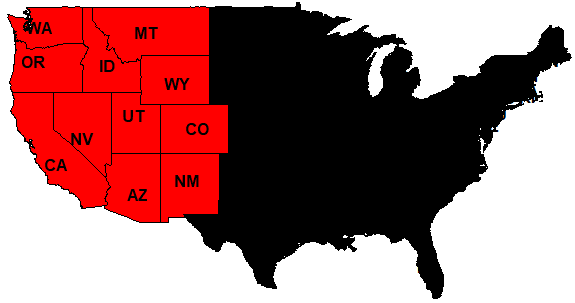
\includegraphics[width=0.5\textwidth]{WesternStatesNoTitleCropped.png} %
\caption{\label{fig:Map11States}Map of 11-state study area.} % The text after \label{} is what shows up as the caption. Inside the brackets for \label{} is just for linking figures to text and is analogous to the AuthorYear in citations. 
\end{figure} % end figure float

%\subsubsection{Acute Impacts of \texorpdfstring{PM\textsubscript{2.5}}{} from Prescribed Fires versus Wildfires on Cardiovascular and Respiratory Health Outcomes}
\subsubsection{Acute Impacts of PM2.5 from Prescribed Fires versus Wildfires on Cardiovascular and Respiratory Health Outcomes}

example analysis with lags \cite{Anyenda2016}

We will analyze the association between acute exposures to PM\textsubscript{2.5} attributed to wildfires and prescribed fires and specific respiratory and cardiovascular health outcomes (see %\nameref{sec:HealthDataSource} 
(Section \ref{sec:HealthDataSource}) for list of outcomes and ICD-9 codes) among Medicare enrollees using a time-stratified case-crossover design using conditional logistic regression with unconstrained distributed lags \cite{Crooks2016,Jaakkola2003, Schwartz2000,Maclure1991}. PM\textsubscript{2.5} exposures will be linked to each Medicare hospital claim by the date of the event (and the corresponding lag days and control days) and home ZIP code of the Medicare enrollee. 

In case-crossover design, each individual serves as their own control, which inherently controls for potential confounding variables, such as age, sex, smoking status, and SES, that do not change within an individual over a short period of time \cite{Maclure1991}. Following the example of \cite{Crooks2016}, we will use a time-stratified approach \cite{LevyReferent2001} for choosing control days. A time-stratified approach chooses the control days to be the same days of the week within the same month and year as the case day and the corresponding lag (0-5) days. Choosing control days as the same day of the week, month and year adjusts for day-of-week effects, seasonality, 
and  long-term trends in the data. We will estimate the effects of PM\textsubscript{2.5} from each fire type, separately and in mutually-adjusted models, on respiratory and cardiovascular hospital admissions at the ZIP code-level across the western US for a seven-year time frame (2008-2014). Although the case-crossover design inherently controls for individual-level confounders that do not change over a short period of time, and the time-stratified controls adjust for day-of-week effects, seasonality, and  long-term trends in the data, we will also adjust for other variables that could be influencing respiratory and cardiovascular outcomes that vary spatially and temporally such as temperature, relative humidity, and ozone. 

As stated in the previous section, the emissions estimates during the NEI years of 2008, 2011, and 2014 used a more sophisticated and accurate methodology. As these emissions estimates are used in the CAMx model that is used to estimate PM\textsubscript{2.5} attributable to each fire type, the fire-attributed exposure estimates in those years may be more accurate than in intervening years. We will therefore additionally run our health analyses for those years with better data (2008, 2011, and 2014) as a sensitivity analysis. 

%what do you think of how I wrote this up about measurement error?
There is growing concern in environmental epidemiology regarding the use of exposure estimates from models rather than measured observations because those models have some error in them that is not accounted for in the epidemiological analysis \cite{samoli_incorporating_2017}. Due to the sparseness of the monitoring network, measured observations alone cannot be used to  estimate air pollution concentrations, particularly in rural areas, see Figure %\ref{fig:MapLocations}
. A few papers have tried to adjust for exposure measurement error using various techniques, none of which has been proven to be the `best' way to account for measurement error in epidemiological studies. Although the results of adjustment for measurement error in these studies were mostly similar to unadjusted methods \cite{samoli_incorporating_2017}, we plan to explore adjustment for exposure measurement error in both the acute and cumulative analyses through the non-parametric bootstrap \cite{Keller2017} or regression calibration \cite{HartAssociation2015}.

Case-crossover designs are considered equivalent to time series methods when they use conditional logistic regression \cite{LuEquivalence2007}. While they are less statistically powered, the time-stratified approach we will use has greater statistical power and less bias than other designs \cite{CarracedoMartinez2010}. There is no formal method of doing power calculations for case-crossover studies, but we anticipate that our estimated sample size for asthma hospitalizations (a very sensitive health outcome associated with wildfire PM\textsubscript{2.5} \cite{Reid2016EHP}) 
of over 8,700 per year, yielding an estimated 61,000 over the 7-year time period, is large enough to detect an effect because it is a larger sample size than used in many other air pollution - health effects studies that used case-crossover design that observed significant associations. For example, \cite{Crooks2016} analyzed dust storms in relation to 49,427 mortality records, and \cite{Haikerwal2015} found a significant association between out-of-hospital cardiac events and PM\textsubscript{2.5} during a wildfire event in Australia with %only 
457 observations. 

%Melissa, please let me know what you think of this. 
%Although there is a recent paper to have investigated the association between wildfire PM\textsubscript{2.5} and cardiorespiratory health among the Medicare population \citep{Liu2016}, our proposed analyses are different from that study in investigating exposures at the ZIP code rather than county level, and in attributing the PM\textsubscript{2.5} to fire types with a much more sophisticated exposure modeling strategy that blends Earth observations with air quality models rather than using air quality modeling alone. Additionally, our study focuses on different years (2008-2014) than their study (2004-2009).
Although there is a recent paper that also investigated the association between wildfire PM\textsubscript{2.5} and cardiorespiratory health among the Medicare population \cite{liu_wildfire-specific_2016}, our proposed analyses are different from that study because we are: (1) investigating potential differential health effects of smoke due to wildfires versus prescribed fires, (2) attributing the PM\textsubscript{2.5} to fire with a much more sophisticated exposure modeling strategy that blends Earth observations with air quality models rather than using air quality modeling alone, (3) investigating exposures at the ZIP code rather than county level, and (4) focusing on different years (2008-2014) from their study (2004-2009).

%\subsubsection{Cumulative Impacts of \texorpdfstring{PM\textsubscript{2.5}}{} from Prescribed Fires versus Wildfires on Cardiovascular and Respiratory Health Outcomes}

\subsubsection{Cumulative Impacts of PM2.5 from Prescribed Fires versus Wildfires on Cardiovascular and Respiratory Health Outcomes}

We will use Poisson regression, or if the data is overdispersed, negative binomial regression \cite{RabeHesketh2008,Kleinbaum1982} to estimate the association between repeated exposure to smoke from prescribed fires and wildfires, separately and in mutually-adjusted models, with respiratory and cardiovascular outcomes. The goal of this analysis is to assess if there are higher rates of respiratory and cardiovascular health outcomes for individuals who have been exposed to smoke repeatedly compared to those with less frequent exposures. We will use the Huber-White sandwich estimator to obtain standard errors robust to model misspecification \cite{freedman_so-called_2006}. For each individual in the Medicare data, we will count the number of cardiovascular and respiratory events (hospitalizations) both in aggregate and for each ICD-9 code separately over the 7-year study period (2008-2014). See %\nameref{sec:HealthDataSource} 
(Section \ref{sec:HealthDataSource}) for list of outcomes and ICD-9 codes included in this study. These counts will be merged with cumulative exposure estimates that take into account both the frequency and intensity of exposure during the study period. Example cumulative exposure estimates are: (1) number of days during the study period with exposure to PM\textsubscript{2.5} from prescribed fires between half the National Ambient Air Quality Standard (NAAQS) for PM\textsubscript{2.5} and NAAQS, (2) number of days during study period with exposure to PM\textsubscript{2.5} from prescribed fires between NAAQS and 1.5*NAAQS, (3) number of days during study period with exposure to PM\textsubscript{2.5} from prescribed fires greater than 1.5*NAAQS, (4) analogous measures for exposure to wildfire smoke, and (5) analogous measures for exposure to the remainder PM\textsubscript{2.5} that is not attributed to either prescribed 
fires 
or wildfires. We will do sensitivity analyses with a variety of PM\textsubscript{2.5} concentration cut points.

In the analysis of repeated exposures to prescribed fires and wildfires, we will control for confounding from several variables including age, sex, and race. We will control for loss to follow-up due to death or migration where data is available by adjusting the person-time of those individuals accordingly. As the Medicare dataset does not have information on individual-level SES variables, we will control for community-level SES, such as ZIP code poverty rates or median income, from the American Community Survey five-year rolling averages for the years ending in 2009-2014 for all ZIP Code Tabulation Areas (ZCTA) in the analysis \cite{ACS2017}. Similarly, we will not have individual-level information on smoking and will adjust for this through estimates of ZIP code-level smoking prevalence rates \cite{OrtegaHinojosaDeveloping2014}. We will also adjust for urban/rural status with an indicator variable by ZIP code from the US Census designations of urban/rural. We will control for potential confounding by ozone using output for that pollutant from CAMx. 

%what do you think, Melissa?
According to the Dartmouth Atlas of Healthcare (http://www.dartmouthatlas.org/data/region/), in 2014 there were over 7,600,000 Medicare enrollees in our study region. A previous study of the Medicare population and health outcomes associated with fire had 5 million enrollees and was able to find a statistically significant 7.2\% (95\% confidence interval: 0.25\%, 15\%) increase in respiratory hospitalizations associated with days with PM\textsubscript{2.5} above 35 [fix units]%\textmu g/m\textsuperscript{3} 
\cite{liu_wildfire-specific_2016}. 
With more enrollees, our study should have the power to detect significant associations should they exist.

\subsubsection{Creation of Indicators of Air Quality and Health Burden from Prescribed Fires Versus Wildfires}
The results of our analyses will influence decision-making by our state partners that are part of WESTAR and EPHTN. In addition to meeting with them in person to present the findings of our analysis, we will also be providing them with data that will be used in their activities in smoke management and public health interventions and messaging, respectively. 

EPHTN has national and state web portals that provide maps and data on environmental and health indicators that can be used by researchers, public health practitioners, and the public to understand the association between environmental exposures and health (see  https://ephtracking.cdc.g % broke up the link so it won't run off the page
ov/DataExplorer/ and https://ephtracking.cdc.gov/showStateTracking). We will calculate monthly, seasonal, and annual averages of total PM\textsubscript{2.5} and PM\textsubscript{2.5} attributed to each type of fire, for each year, by county. These will be given to each of the seven states in our region who are in EPHTN and also to the other four states in our region if they are interested. 

The state air quality managers who are part of WESTAR and the state public health officials of EPHTN plan to use the information about health impacts of prescribed fire PM\textsubscript{2.5} in their decision-making. We will have regular phone conferences with these stakeholders throughout the duration of the grant, providing them with updates on our progress, and obtaining their feedback. We will also present our results in years 2 and 3 of this grant at conferences to which the partners attend such as the annual business meetings for EPHTN and WESTAR.

\section{Performance Measures}
% 1 page
% This section must articulate the metrics and measures (both quantitative and qualitative) the team will use to determine the outcomes, results, and value of the project. The measures should, at a minimum, include those that the partner/end user/decision-making organization(s) employ to assess their decision making and services as well as those used to establish the baseline performance.
%Strategically timed calls with end users to ensure we are progressing towards products that they will use in their decision-making

%%Melissa, let's discuss the clarity of this section tomorrow.

During our project kick-off meeting, partners from state air quality and public health departments will present about their respective state-specific baseline performance measures on decision-making related to prescribed fires and wildfires. This will allow us to benchmark current decision-making processes, identify difficulties in communicating across state-level bureaucracy, and identify what information is limiting their decision-making. These states have already identified that a lack of information on health impacts associated with prescribed fires means that they are making decisions based on the assumption that the levels of PM\textsubscript{2.5} denote where health impacts occur, but that empirical evidence for historical fires could help inform or improve those decisions. 

Some of the state partners have already provided us with information on how they currently measure performance related to fire smoke. For example, the department of health in Washington measures baseline performance as the levels of PM\textsubscript{2.5} and the number of deaths, hospitalizations, and emergency department visits for respiratory and cardiovascular health endpoints on days with smoke. New Mexico is trying to allow more prescribed fires in their interagency smoke coordination and communication plan that they review annually, but they get pushback from the public with many complaints about prescribed fire planning and smoke levels. They plan to measure baseline as the number of complaint calls to the department of health and the environment department and then see if those numbers change after providing information to the public from our proposed project about associations between air pollution from prescribed fires and wildfires and respiratory and cardiovascular health. 

For our project, we will use the following measures to denote performance: (1) how much does each agency use empirical information of the health impacts of fires for their decision-making, and (2) how well do the public health and air quality managers in a given state collaborate/communicate with each other related to their decision-making related to prescribed and wildfires. We will assess this repeatedly through the project. Therefore, we will be at an ARL 3 (detailed characterization of the user decision-making process completed) by the end of the first quarter of the grant, having started at ARL 2 (decision-making activity to be enhanced by the application identified). 

In each annual meeting with the state partners, we will assess the extent to which they are using health-based information in their smoke decision-making and that the results from our investigations are influencing those decisions. We hope to be at ARL 4 by the end of year 1 of the grant, and getting to ARL 7 by the end of the project. This will be demonstrated by states proving that they are using information on the health impacts of prescribed fires in their smoke management plans and in their public health messaging during such fires. To get beyond ARL 7 we recognize will require further funding, which our group hopes to pursue during the third year of this grant such that the decision-making activity can be further enhanced with more health information. By engaging with our state-level health partners, we expect to learn more about their needs in order to contribute to a sustained decision-making process.

\subsubsection{Measurement error}

[Consider accounting for measurement error via a nonparametric bootstrap, see \cite{Keller2017}. Also consider spatial compatibility - ``monitor and cohort locations are sampled from identical, or at least very similar, spatial distributions'']

%Suspendisse viverra eleifend nulla at facilisis. Nullam eget tellus orci. Cras sit amet lorem velit. Maecenas rhoncus pellentesque orci eget vulputate. Phasellus massa nisi, mattis nec elementum accumsan, blandit non neque. In ac enim elit, sit amet luctus ante. Cras feugiat commodo lectus, vitae convallis dui sagittis id. In in tellus lacus, sed lobortis eros. Phasellus sit amet eleifend velit. Duis ornare dapibus porttitor. Maecenas eros velit, dignissim at egestas in, tincidunt lacinia erat. Proin elementum mi vel lectus suscipit fringilla. Mauris justo est, ullamcorper in rutrum interdum, accumsan eget mi. Maecenas ut massa aliquet purus eleifend vehicula in a nisi. Fusce molestie cursus lacinia.

% \begin{definition}
% A bounded function $\theta$ is a weak solution of QG if for any
% $\phi\,\epsilon\,
% C_0^{\infty}(\fdb\times\mathbb{R}\times[0,\vep])$ we have
% \begin{eqnarray}
% &&  \int_{\mathbb{R}^+\times\fd\times\mathbb{R}} \hspace{-25pt}
%  \theta(x,y,t)\, \pr_t \phi
% \,(x,y,t) dy dx dt+\nonumber\\
%   & +&\int_{\mathbb{R}^+\times\fd\times\mathbb{R}}
% \hspace{-26pt} \theta\,(x,y,t) u(x,y,t)\cdot\nabla\phi\,(x,y,t)
% dydxdt = 0 \label{weaksol} \end{eqnarray}
% where $u$ is determined previously.
% \end{definition}

% Vestibulum ante ipsum primis in faucibus orci luctus et ultrices posuere cubilia Curae; Mauris eu sapien nunc, sit amet accumsan dui. Nulla ac diam ut nunc placerat semper eget et libero. Vestibulum ante ipsum primis in faucibus orci luctus et ultrices posuere cubilia Curae; Cras hendrerit ullamcorper sapien vitae luctus. Quisque vel diam massa. Vestibulum dui nibh, facilisis vel vestibulum eu, viverra in quam.

% \begin{theorem}
% If the active scalar $\theta$ satisfies
% the equation \eqref{weaksol}, then $\varphi$ satisfies the equation
% \begin{eqnarray}
% \mfrac{\pr \varphi}{\pr t}(x,t)&=&\hspace{-2pt}\dst
% \int_{\fd}\mfrac{\mfrac{\pr \varphi}{\pr x}(x,t)-\mfrac{\pr
% \varphi}{\pr
% u}(u,t)}{[(x-u)^{2}+(\varphi(x,t)-\varphi(u,t))^{2}]^{\f12}}\nonumber\\
% &&
% \chi(x-u,\varphi(x,t)-\varphi(u,t)) du \hspace{3pt} +
% \nonumber\\
% &+&\dst \int_{\fd} \Big{[}\mfrac{\pr \varphi} {\pr
% x}(x,t)-\mfrac{\pr \varphi}{\pr u} (u,t)\Big{]}
% \nonumber\\&&
% \eta(x-u,\varphi(x,t)-\varphi(u,t)) du + Error
% \end{eqnarray}
% with $|Error|\leq C\, \delta | log\delta| $ where $C$ depends only
% on $\|\theta\|_{L^{\infty}}$ and $\|
% \nabla\varphi\|_{L^{\infty}}$.
% \end{theorem}

% Class aptent taciti sociosqu ad litora torquent per conubia nostra, per inceptos himenaeos. Integer accumsan ornare tortor at varius. Phasellus ullamcorper blandit dolor sit amet tempus. Curabitur ligula urna, ultrices in iaculis eu, eleifend vel urna. Praesent ullamcorper imperdiet purus, ut interdum sem interdum dictum. Proin euismod volutpat eros ac mattis. Quisque sit amet massa ac tortor cursus malesuada at vitae nisi. Nam quis neque et nunc vehicula cursus sit amet at tellus.
\end{materials}

%----------------------------------------------------------------------------------------
%	APPENDICES (OPTIONAL)
%----------------------------------------------------------------------------------------

\appendix
An appendix without a title.

\appendix[Appendix title]
An appendix with a title.

%----------------------------------------------------------------------------------------
%	ACKNOWLEDGEMENTS
%----------------------------------------------------------------------------------------

\begin{acknowledgments}
This work was partially supported by a grant from the Spanish Ministry of Science and Technology.
\end{acknowledgments}

%----------------------------------------------------------------------------------------
%	BIBLIOGRAPHY
%----------------------------------------------------------------------------------------

%% PNAS does not support submission of supporting .tex files such as BibTeX.
%% Instead all references must be included in the article .tex document. 
%% If you currently use BibTeX, your bibliography is formed because the 
%% command \verb+\bibliography{}+ brings the <filename>.bbl file into your
%% .tex document. To conform to PNAS requirements, copy the reference listings
%% from your .bbl file and add them to the article .tex file, using the
%% bibliography environment described above.  

%%  Contact pnas@nas.edu if you need assistance with your
%%  bibliography.

% Sample bibliography item in PNAS format:
%% \bibitem{in-text reference} comma-separated author names up to 5,
%% for more than 5 authors use first author last name et al. (year published)
%% article title  {\it Journal Name} volume #: start page-end page.
%% ie,
% \bibitem{Neuhaus} Neuhaus J-M, Sitcher L, Meins F, Jr, Boller T (1991) 
% A short C-terminal sequence is necessary and sufficient for the
% targeting of chitinases to the plant vacuole. 
% {\it Proc Natl Acad Sci USA} 88:10362-10366.


%% Enter the largest bibliography number in the facing curly brackets
%% following \begin{thebibliography}

%\bibliography{ReidGroupReferences}

\bibliographystyle{plain}
\bibliography{ReidGroupReferences}

% \begin{thebibliography}{10}
% \bibitem{BN}
% M.~Belkin and P.~Niyogi, {\em Using manifold structure for partially
%   labelled classification}, Advances in NIPS, 15 (2003).

% \bibitem{BBG:EmbeddingRiemannianManifoldHeatKernel}
% P.~B\'erard, G.~Besson, and S.~Gallot, {\em Embedding {R}iemannian
%   manifolds by their heat kernel}, Geom. and Fun. Anal., 4 (1994),
%   pp.~374--398.

% \bibitem{CLAcha1}
% R.R.~Coifman and S.~Lafon, {\em Diffusion maps}, Appl. Comp. Harm. Anal.,
%   21 (2006), pp.~5--30.

% \bibitem{DiffusionPNAS}
% R.R.~Coifman, S.~Lafon, A.~Lee, M.~Maggioni, B.~Nadler, F.~Warner, and
%   S.~Zucker, {\em Geometric diffusions as a tool for harmonic analysis and
%   structure definition of data. {P}art {I}: Diffusion maps}, Proc. of Nat.
%   Acad. Sci.,  (2005), pp.~7426--7431.

% \bibitem{Clementi:LowDimensionaFreeEnergyLandscapesProteinFolding}
% P.~Das, M.~Moll, H.~Stamati, L.~Kavraki, and C.~Clementi, {\em
%   Low-dimensional, free-energy landscapes of protein-folding reactions by
%   nonlinear dimensionality reduction}, P.N.A.S., 103 (2006), pp.~9885--9890.

% \bibitem{DoGri}
% D.~Donoho and C.~Grimes, {\em Hessian eigenmaps: new locally linear
%   embedding techniques for high-dimensional data}, Proceedings of the National
%   Academy of Sciences, 100 (2003), pp.~5591--5596.

% \bibitem{DoGri:WhenDoesIsoMap}
% D.~L. Donoho and C.~Grimes, {\em When does isomap recover natural
%   parameterization of families of articulated images?}, Tech. Report Tech. Rep.
%   2002-27, Department of Statistics, Stanford University, August 2002.

% \bibitem{GruterWidman:GreenFunction}
% M.~Gr\"uter and K.-O. Widman, {\em The {G}reen function for uniformly
%   elliptic equations}, Man. Math., 37 (1982), pp.~303--342.

% \bibitem{Simon:NeumannEssentialSpectrum}
% R.~Hempel, L.~Seco, and B.~Simon, {\em The essential spectrum of neumann
%   laplacians on some bounded singular domains}, 1991.

% \bibitem{1}
% Kadison, R.\ V.\ and Singer, I.\ M.\ (1959)
% Extensions of pure states, {\it Amer.\ J.\ Math.\ \bf
% 81}, 383-400.

% \bibitem{2}
% Anderson, J.\ (1981) A conjecture concerning the pure states of
% $B(H)$ and a related theorem. in {\it Topics in Modern Operator
% Theory}, Birkha\"user, pp.\ 27-43.

% \bibitem{3}
% Anderson, J.\ (1979) Extreme points in sets of
% positive linear maps on $B(H)$. {\it J.\ Funct.\
% Anal.\
% \bf 31}, 195-217.

% \bibitem{4}
% Anderson, J.\ (1979) Pathology in the Calkin algebra. {\it J.\
% Operator Theory \bf 2}, 159-167.

% \bibitem{5}
% Johnson, B.\ E.\ and Parrott, S.\ K.\ (1972) Operators commuting
% with a von Neumann algebra modulo the set of compact operators.
% {\it J.\ Funct.\ Anal.\ \bf 11}, 39-61.

% \bibitem{6}
% Akemann, C.\ and Weaver, N.\ (2004) Consistency of a
% counterexample to Naimark's problem. {\it Proc.\ Nat.\ Acad.\
% Sci.\ USA \bf 101}, 7522-7525.

% \bibitem{TSL}
% J.~Tenenbaum, V.~de~Silva, and J.~Langford, {\em A global geometric
%   framework for nonlinear dimensionality reduction}, Science, 290 (2000),
%   pp.~2319--2323.

% \bibitem{ZhaZha}
% Z.~Zhang and H.~Zha, {\em Principal manifolds and nonlinear dimension
%   reduction via local tangent space alignement}, Tech. Report CSE-02-019,
%   Department of computer science and engineering, Pennsylvania State
%   University, 2002.
% \end{thebibliography}

%----------------------------------------------------------------------------------------

\end{article}

%----------------------------------------------------------------------------------------
%	FIGURES AND TABLES
%----------------------------------------------------------------------------------------

%% Adding Figure and Table References
%% Be sure to add figures and tables after \end{article}
%% and before \end{document}

%% For figures, put the caption below the illustration.
%%
%% \begin{figure}
%% \caption{Almost Sharp Front}\label{afoto}
%% \end{figure}

\begin{figure}[h]
\centerline{
\includegraphics[width=0.4\linewidth]{placeholder.jpg}}
\caption{Figure caption}\label{placeholder}
\end{figure}

%% For Tables, put caption above table
%%
%% Table caption should start with a capital letter, continue with lower case
%% and not have a period at the end
%% Using @{\vrule height ?? depth ?? width0pt} in the tabular preamble will
%% keep that much space between every line in the table.

%% \begin{table}
%% \caption{Repeat length of longer allele by age of onset class}
%% \begin{tabular}{@{\vrule height 10.5pt depth4pt  width0pt}lrcccc}
%% table text
%% \end{tabular}
%% \end{table}

\begin{table}[h]
\caption{Table caption}\label{sampletable}
\begin{tabular}{l l l}
\hline
\textbf{Treatments} & \textbf{Response 1} & \textbf{Response 2}\\
\hline
Treatment 1 & 0.0003262 & 0.562 \\
Treatment 2 & 0.0015681 & 0.910 \\
Treatment 3 & 0.0009271 & 0.296 \\
\hline
\end{tabular}
\end{table}

%% For two column figures and tables, use the following:

%% \begin{figure*}
%% \caption{Almost Sharp Front}\label{afoto}
%% \end{figure*}

%% \begin{table*}
%% \caption{Repeat length of longer allele by age of onset class}
%% \begin{tabular}{ccc}
%% table text
%% \end{tabular}
%% \end{table*}

%----------------------------------------------------------------------------------------

\section{Ideas and Notes for paper}

See this paper for discussion of changes in toxicity of smoke between smoldering/open flame: Kim YH, Tong H, Daniels M, Boykin E, Krantz QT, McGee J, et al.
Cardiopulmonary toxicity of peat wildfire particulate matter and the predictive
utility of precision cut lung slices. Part Fibre Toxicol. 2014;11(1):1–17.

Discuss errors/uncertainties in assigning exposure data in health studies: (references in Linares et al., 2018 \cite{linares_impact_2018}
\begin{enumerate}
\item Weichenthal, S., Kulka, R., Lavigne, E., van Rijswijk, D., Brauer,M., Villeneuve, P.J., Stieb, D.,
Joseph, L., Burnett, R.T., 2017. Biomass burning as a source of ambient fine particulate
air pollution and acute myocardial infarction. Epidemiology 28 (3), 329–337 (May). \url{https://insights.ovid.com/crossref?an=00001648-201705000-00005}

\item Ingebrigtsen, R., Steinsland, I., Cirera, L1., Saez, M., 2015. Spatially misaligned data and the
impact of monitoring network on health effect estimates (Doctoral thesis at NTNU).
In: Ingebrigtsen, R. (Ed.), Bayesian Spatial Modelling of Non-stationary Processes
and Misaligned Data Utilising Markov Properties for Computational Efficiency. Norwegian
University of Science and Technology. 
\end{enumerate}

Re-read \cite{jones_application_2017}, ``Finally, prescribed burning presents a dilemma for the rational policymaker. While it can reduce fuel loads and lessen the intensity of future wildfires, it also creates immediate smoke effects and associated costs. Considering this tradeoff is important given the significant consequences of smoke exposure.''

Read Haikerwal et al \url{http://dx.doi.org/10.1080/10962247.2015.1032445}

Read Liu et al., 2015 \url{http://dx.doi.org/10.1016/j.envres.2014.10.015}

Read Fantke et al, 2015 \cite{http://dx.doi.org/10.1007/s11367-014-0822-2}

Read Hanninen et al 2009 \cite{http://dx.doi.org/10.1038/jes.2008.31}

Read Williamson GJ, Bowman DMJS, Price OF, Henderson SB, Johnston FH (in press) A transdisciplinary approach to understanding the health effects of wildfire and prescribed fire smoke regimes. Environmental Research Letters . (cited in \cite{hyde_air_2017}

 % place to put notes and ideas for paper. Will need to be commented.

%----------------------------------------------------------------------------------------
\end{document}